\pdfoutput=1

\documentclass{l4proj}

%
% put any packages here
%
\usepackage{url}

\begin{document}
\title{GEMS: Glasgow Energy Measurement System for the Raspberry Pi Cloud}
\author{Piotr Hosa}
\date{\today}
\maketitle

\begin{abstract}

\end{abstract}

\renewcommand{\abstractname}{Acknowledgements}
\begin{abstract}

\end{abstract}

\educationalconsent
%
%NOTE: if you include the educationalconsent (above) and your project is graded an A then
%      it may be entered in the CS Hall of Fame
%
\tableofcontents
%==============================================================================

\chapter{Introduction}
\pagenumbering{arabic}

\section{Motivation}
Cloud technology has become increasingly popular in recent years. Owners of large infrastructures such as Google, Amazon and Microsoft are able to offer their customers highly scalable services at a lowering cost and no upfront investment. However, dealing with considerable amounts of data and traffic invokes a need for sizeable hardware, which imposes various challenges on its owners. These challenges include automated service provisioning, virtual machine migration and energy management among others \cite{zhang_cheng_boutaba_2010}.

\noindent
The Glasgow Raspberry Pi Cloud (RPC), as discussed in section \ref{the_glasgow_picloud}, is a scale model data centre. The RPC is a research and educational tool and it aims to mimic full-sized cloud infrastructures. This is incrementally achieved by the projects done on the RPC, which use leading virtualisation and cloud software such as Docker and Kubernetes.

\noindent
This project focuses on developing a power monitoring system for the RPC, which is a fundamental step toward power management. Monitoring makes it possible to identify machines with abnormal power consumption, but also to compare the power efficiency of similar software frameworks. While power management is not of particular concern in a cluster of this size, implementing such a system advances the project by making the RPC more similar to full-scale data centres. In the full-scale cases energy management is highly important. Not only is it crucial for reducing operational costs but also to keeping in accordance with environmental concerns, which will only increase in the future \cite{dabbagh_hamdaoui_guizani_rayes_2015}.

\section{The Glasgow Raspberry Pi Cloud}
\label{the_glasgow_picloud}
\subsection{Overview}
The Raspberry Pi project at the University of Glasgow was started in 2012 by a group of researchers in the School of Computing Science. The motivation to pursue the project was a lack of satisfactory methods that would have allowed to conduct research on data centres and cloud computing. Before the Raspberry Pi Cloud, recreating such infrastructures relied mainly on software simulations and using physical environments with a very limited number of machines. Both of these methods were aimed at reducing costs of such research systems. The RPC eliminated the financial overhead by using 56 low-cost computers and therefore allowed to model full-scale data centres more closely. Using Raspberry Pis in the project also eliminated other challenges associated with traditional data centre servers like space constraints, cooling and considerable energy used by the machines. The RPC also has the advantage of exhibiting real network traffic and running real cloud services, which is difficult to model in software simulations \cite{tso_white_jouet_singer_pezaros_2013}.

\subsection{The Original Cloud}
In its original version the RPC consisted of 4 racks of 14 Raspberry Pi 1 Model B computers. Each rack had a top-of-rack switch that connected to a central OpenFlow switch and then to the Internet. There was also a master node also connected to the OpenFlow switch that for system management. Each of the nodes in the rack run the Raspbian version of Debian. The first software developed for the cluster was a REST API with a web interface. The project also involved experimenting with LXC virtualisation, Hadoop and Software Defined Networking \cite{white_2013}.

\subsection{More Recent Projects}
One of the most recent projects with the RPC involved a hardware upgrade. One rack of 14 computers was fitted with Raspberry Pi 2 Model B devices, which are more powerful than the ones used previously. The new infrastructure extended the potential applications of the cluster and made it possible to experiment with Kubernetes, Google's cluster management software. In the recent months Kubernetes has been adapted to the ARM architecture of the Raspberry Pi \cite{walker_2015} and work has been done on the Kubernetes Dashboard \cite{mcwha_2016}.

\noindent
Before the upgrade, a team of students worked on a wake-on-LAN hardware and load balancer software for the cluster, which used Docker and SaltStack.

\section{Related Work}
\subsection{Raspberry Pi Clusters}
Since the Raspberry Pi has been released it became hugely popular in the computing community. This meant that not only the researchers at the University of Glasgow, but also other research institutions took advantage of the low-cost computers. 

* A Low-Cost Computer Cluster for High-Performance Computing Education\\
*Affordable and Energy-Efficient Cloud Computing Clusters: The Bolzano Raspberry Pi Cloud Cluster Experiment\\
*Iridis-pi: a low-cost, compact demonstration cluster\\
\subsection{Power Measurement}
The core element of hardware in this project is the power measuring shield created by the MAGEEC project at the University of Bristol. The shield attaches to the I/O pins of the STM32F4 Discovery board and provides hardware interfaces for measuring up to 3 external sources. The STM board does not have an operating system and it uses pre-loaded C programs that run continuously when power is supplied to the board. The shield was designed with the purpose of measuring the power efficiency of compilers. Therefore the processors that are measured in the MAGEEC project require to be embedded in boards with jumper pins that allow to intercept the CPU power supply or to be stand-alone processors such as ATMEGA AVRs. This served the purpose of measuring the power consumption of the CPU only, excluding other components on the board. In this project the author uses the STM board to measure the power consumption of all the components in the Raspberry Pi, therefore the lack of CPU jumper pins does not pose an obstacle that would otherwise exclude the Raspberry Pi of being subject to this experiment.

*PowerPi: Measuring and Modeling the Power Consumption of the Raspberry Pi\\
*A Study Case of Restful Frameworks in Raspberry Pi: A Perfomance and Energy Overview\\
*Impact of different compiler options on energy consumption\\
*Energy Measurement Infrastructure\\

%==============================================================================
\chapter{Requirements}

\section{Use Cases}
Users can
\begin{enumerate}
	\item See overview of data from cluster in graphs/tables
	\item See overview of cluster as heatmap
	\item Obtain CSV files to analyse data in more detail
\end{enumerate}
\section{Functional Requirements}
\begin{enumerate}
	\item Table with requirements
	\item User stories in appendix(?)
\end{enumerate}
\section{Non-Functional Requirements}
\begin{enumerate}
	\item Accessibility
	\item Compatibility (plug and play)
	\item Recoverability (broken connections, API down)
	\item Performance (multiple users can access without over-stressing the system)
\end{enumerate}

%==============================================================================
\chapter{Design}
\begin{figure}[!ht]
  \caption{System diagram demonstrating the power component of the system.}
  \centering
    \includegraphics[width=0.5\textwidth]{figures/power_arch}
\end{figure}
\section{Hardware}
\begin{enumerate}
	\item Adapted from the MAGEEC project
	\item The setup in the Glasgow PiCloud (MAGEEC wires + network)
\end{enumerate}
\begin{figure}[!ht]
  \caption{Basic wiring set-up for measuring power consumption.}
  \centering
    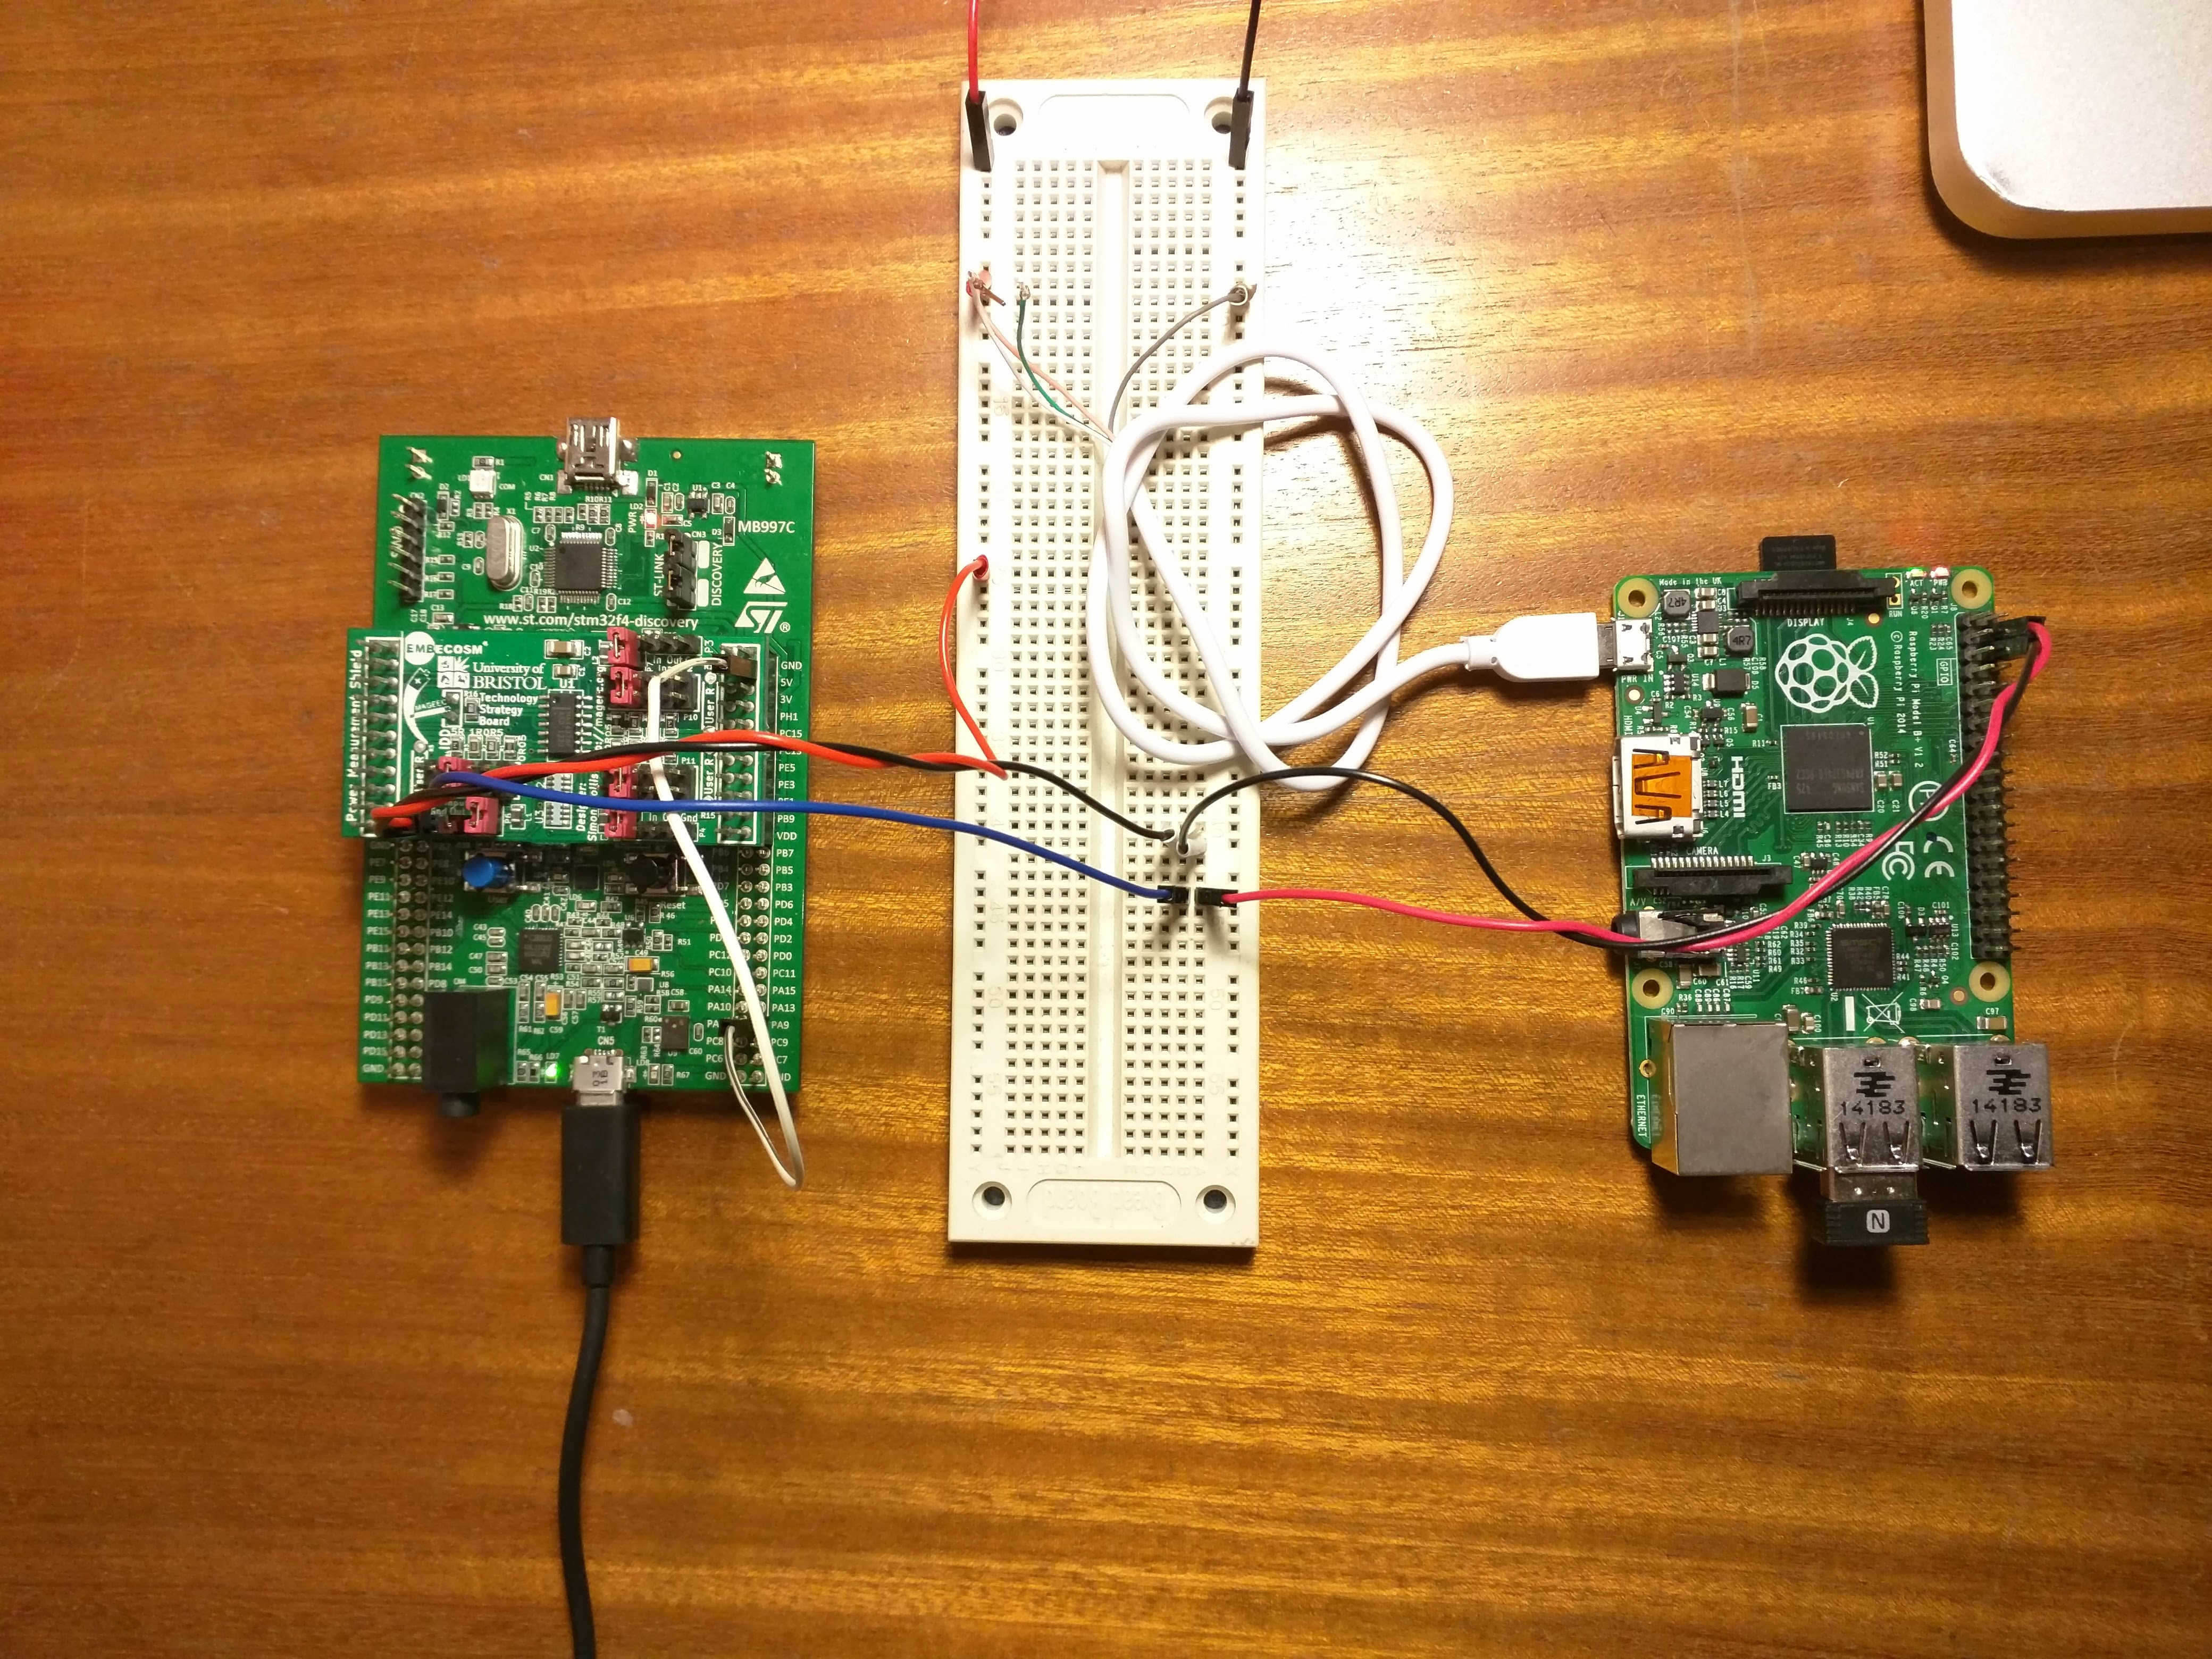
\includegraphics[width=0.5\textwidth]{figures/init_setup}
\end{figure}
\section{API Server}
\begin{enumerate}
	\item Choice of OS for the Pi
	\item Python chosen as it is most frequently used on the Pi and therefore there is a lot of support and documentation for it.
	\item Flask (and Flask restless) chosen for API. Other options available (Django, Tastypy and Sadman) but Flask is simple and popular and therefore seemed like the right choice.
	\item Chose to use SQLite dabase with Flask SQLalchemy to make database access easier.
\end{enumerate}
\section{Web Client}
\begin{enumerate}
	\item Single Page Application design (rendering and logic done in client which takes processing off server; more responsive websites)
	\item There is a number of frameworks available (Ember.js, ExtJS, React, Knockout) but Angular has a large community and it supports bidirectional data binding, which some of the other frameworks lack
	\item Many front-end frameworks have been adapted to Angular but if they have not it is possible to do it by hand.
\end{enumerate}
\begin{figure}[!ht]
  \caption{Dashboard wire frame for the web client}
  \centering
    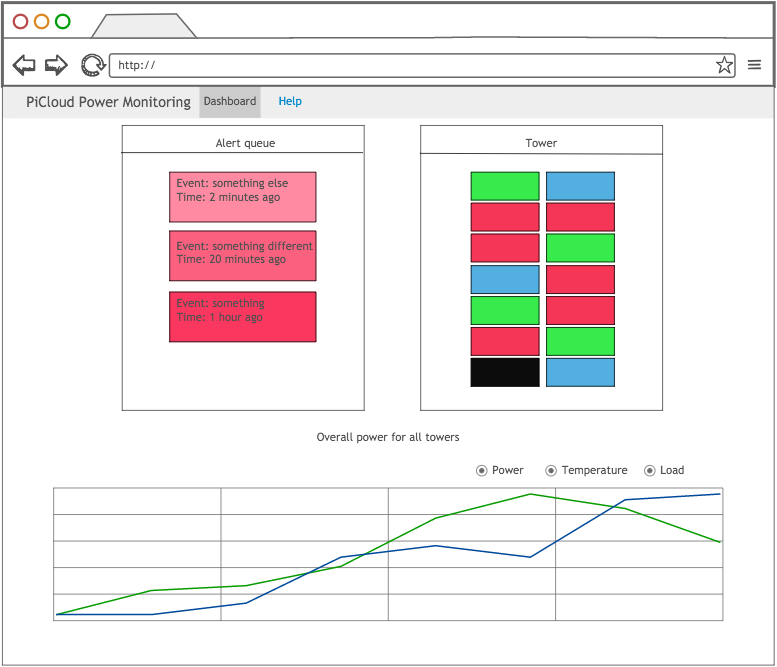
\includegraphics[width=0.5\textwidth]{figures/v2_dashboard}
\end{figure}

%==============================================================================
\chapter{Implementation}
\section{Logger Node}
\begin{enumerate}
	\item Logging python (based on MAGEEC pyenergy library)
	\item Database and API
	\item Web client
	\item Salt managing scripts
\end{enumerate}
\section{Minion Nodes}
\begin{enumerate}
	\item Reporting python
\end{enumerate}

%==============================================================================
\chapter{Evaluation}
\section{Testing}
\begin{enumerate}
	\item Python tests for scripts
	\item JavaScript tests(?)
\end{enumerate}
\section{Acceptance Testing}
\begin{enumerate}
	\item Overview of testing scenario
	\item Feedback from testers
	\item Changes in system based on feedback
\end{enumerate}

%==============================================================================
\chapter{Conclusion}
\section{Summary}
\begin{enumerate}
	\item What has been implemented
	\item What the system can do
	\item Comment on usability
\end{enumerate}
\section{Future Work}
\begin{enumerate}
	\item What other features are the next logical step
	\item How do those features fit within the technology stack
\end{enumerate}



%\vspace{-7mm}
%\begin{figure}
%\centering
%\includegraphics[height=9.2cm,width=13.2cm]{uroboros.pdf}
%\vspace{-30mm}
%\caption{An alternative hierarchy of the algorithms.}
%\label{uroborus}
%\end{figure}

%%%%%%%%%%%%%%%%
%              %
%  APPENDICES  %
%              %
%%%%%%%%%%%%%%%%
\begin{appendices}
\chapter{Appendix}
\end{appendices}
%%%%%%%%%%%%%%%%%%%%
%   BIBLIOGRAPHY   %
%%%%%%%%%%%%%%%%%%%%

\bibliographystyle{plain}
\bibliography{bib}

\end{document}
